
% relevanzwerte und priorität erklären (nicht erklären dass die von
%0-100 gehn und prozente darstellen das erfolgt in schnittstellen)

\todo{anfangs bla find ich noch unschön}
Dieses Kapitel befasst sich mit den Vorbetrachtungen zur Projektarbeit. Dabei
geht es um {\"U}berlegungen zur Fehlererkennung und der Handhabung von
Verbindungsabbr{\"u}chen bzw. fehlerhaften {\"U}bertragungen.

\textbf{Time To Live}

Die TTL bezeichnet die Lebensdauer eines Datenpakets und ist dabei von
unterschiedlichen Aspekten abh{\"a}ngig. So kann ein Paket einerseits nach
Ablauf eines Zeitraums verworfen werden oder aber nach einer bestimmten Anzahl
von hops. \todo{vervollständigende frage was sind hops eventl nebensatz
erklärnug} Unter Ber{\"u}cksichtigung einer Interplanetare Kommunikation
w{\"a}re eine TTL Realisierung per Zeitstempel sinnvoll, da hier{\"u}ber
unrealistische {\"U}bertragungszeiten erkannt werden k{\"o}nnen.
\todo{wir hatten glaub ich schon ein erstes konzept/ideen zur umsetzung}

\textbf{Protocol Stack}

Dieser Abschnitt befasst sich mit der Kommunikation zwischen dem Client
und dem Server (z.B. Station auf der Erde und Rover auf dem Mars). Die
Kommunikation erfolgt hierbei {\"u}ber UDP Sockets. Das im Verlauf der Arbeit
Implementierte CROP Protokoll verpackt zuvor die Inhalte (Bilder, Sensordaten etc.) 
nach den Protokollvorgaben und reicht die Datenpakete aus der priorisierten Queue 
direkt an den zuvor ge{\"o}ffneten UDP Socket weiter. Durch eine Client/Server
basierte Socket-Kommunikation {\"u}ber UDP 
(verbindungslose Kommunikation im Gegensatz zu TCP) wird der Datenstrom an die
definierte Zieladresse und den definierten Zielport geleitet. Da es sich
hierbei um eine UDP Socket-Verbindung handelt, werden Paketverluste nicht
bemerkt (keine Sicherung der Daten{\"u}bertragung). Lediglich ein {\"u}bergreifendes
Protokoll wie CROP, welches dies erkennen k{\"o}nnte, kann dann eine erneute
Sendung anfordern (zum jetzigen Zeitpunkt ist CROP jedoch nicht f{\"a}hig einen
Verbindungsabbruch zu detektieren). Die dabei genutzte Adressierungsart wird im
CROP Protokoll festgelegt und dann f{\"u}r die Socket-Kommunikation {\"u}bernommen. Im
Testszenario der Projektarbeit kam dabei IPv4 zum Einsatz. \todo{wie sieht
unser protocol stack im moment aus?}

\begin{figure}[H]
\centering
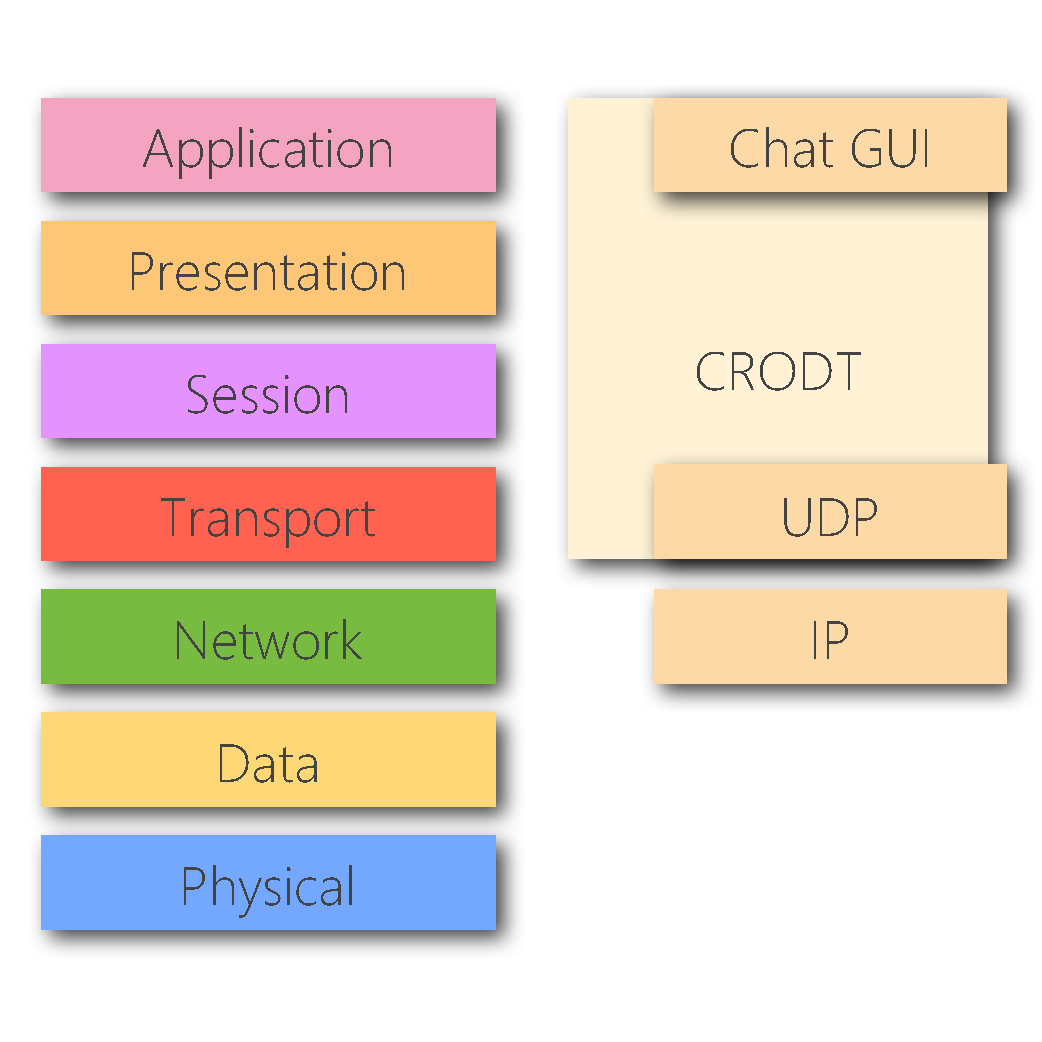
\includegraphics[scale=.38]{OSI.pdf}
\caption{{\"U}berblick des OSI-Schichtenmodells und der Zuordnung von CROP}
\label{fig:OSI}
\end{figure}

\begin{figure}[H]
\centering
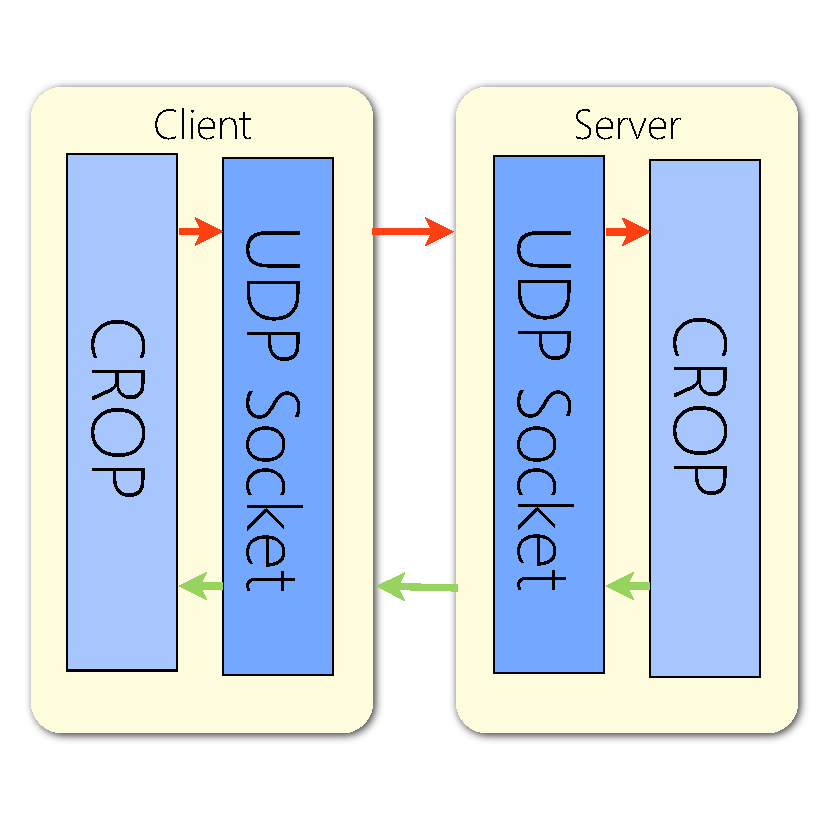
\includegraphics[scale=.5]{UDP_CROP.pdf}
\caption{Client/Server Kommunikation {\"u}ber UDP-Socket}
\label{fig:Socket-Kommunikation}
\end{figure}

\textbf{Error Correction Code}

Zur Fehlererkennung bzw. Korrektur kommt ein CRC-Code zum Einsatz. Dieser kann
innerhalb des Protokolls je nach Paketgr{\"o}{\ss}e auf CRC 16 Bit oder CRC 32
Bit eingestellt werden. Die Pr{\"u}fsumme wird durch einen mathematischen
Algorithmus ermittelt und dann mit dem Paket {\"u}bertragen. Wenn der
Empf{\"a}nger die R{\"u}ckrechnung unter Einbeziehnung der Pr{\"u}fsumme
vornimmt, kann anhand des Ergebnisses ermittelt werden ob das Paket
verf{\"a}lscht wurde. \todo{eventl genauer die beiden CRCs beschreiben? wie die
funktionieren formeln etc?}
